%----------------------------------------------------------------------------
\chapter{Elméleti megalapozás és szakirodalmi áttekintő}
%----------------------------------------------------------------------------

\section {Webes alkalamazás felépítése}

Az F1TM a React JavaScript programozási nyelv keretrendszerével valósult meg a Microsoft Visual Studio Code IDE-ben. Az alkalmazás használ harmadik féltől származó könyvtárakat is, amelyek felgyorsítják a fejlesztési folyamatot, mivel előre le van implementálva számos funkcionalitás. Ezek általában több fejlesztő által vannak használva és tesztelve, ezért többségében gyorsabbak és biztonságosabbak.

Lévén, hogy az alkalmazás egy webes platform, a struktúrája két fő részből áll: frontend és backend. Ezen projekt keretében első sorban a frontend implementációján volt a hangsúly.

A frontend az a része a webes alkalmazásnak, amellyel a felhasználók közvetlenül interakcióba lépnek. Ez a rész felelős a UI megjelenítéséért és a felhasználói interakciók kezeléséért. A frontend általában a böngészőben fut, és a felhasználó által látott elemeket jeleníti meg, például az oldalak, űrlapok, gombok, navigációs elemek stb. A frontend tervezésekor figyelembe kell venni a UX aspektusait is. Ezek azért felelnek, hogy a felhasználói élmény a lehető legjobb legyen a weboldal böngészése során. Itt első sorban a letisztultság, átláthatóság és az összezavaró elemek elkerülése a legfőbb cél.

A frontend technológiák közé tartozhatnak:
\begin{itemize}
	\item HTML: Az alapvető struktúrát és tartalmat határozza meg a weboldalakhoz.
	\item CSS: A megjelenítést és a stílust adja a weboldalaknak, mint például a színek, betűtípusok, elrendezés stb.
	\item JavaScript: A dinamikus és interaktív funkciókért felelős, például animációk, eseménykezelés, adatmanipuláció. Gyakran használnak frontend keretrendszereket, például a React JS-t, Next.js-t vagy Angular-t, amelyek segítenek az alkalmazás fejlesztésében és szervezésében. 
\end{itemize}

A backend a szerveroldali logikát és adatkezelést végzi. Ez a rész felelős az adatbáziskezelésért, a logika végrehajtásáért, a felhasználói kérések feldolgozásáért és a válaszok generálásáért. A backend nem közvetlenül látható vagy interaktív a felhasználók számára, viszont folyamatosan kommunikál a frontend-el az API-kon keresztül.

A backend technológiák közé tartozhatnak:
\begin{itemize}
	\item Szerveroldali programozási nyelvek: Python, Ruby, Java, PHP stb.
	\item Keretrendszerek: Node.js, Django, Ruby on Rails, Laravel stb., amelyek segítenek az alkalmazás fejlesztésében és a szerveroldali logika megvalósításában.
	\item Adatbázis-kezelő rendszerek: MySQL, PostgreSQL, MongoDB stb., amelyek tárolják az alkalmazás adatai és lehetővé teszik ezek lekérdezését és manipulálását.
\end{itemize}

A frontend és backend között kommunikáció történik HTTP kérések és válaszok segítségével. A frontend kéréseket küld a backendnek, például adatlekérdezések vagy műveletek végrehajtása érdekében. Ezek a backend(ek) API végpontjain keresztül történnek A backend feldolgozza ezeket a kéréseket, és visszaküldi a válaszokat a frontendnek (\ref{abra:Architektura}). Nagyobb alkalmazások esetében megtörténhet, hogy a frontend több backend szerverről kéri le az információkat. Ez az felhasználó számára nem feltűnő, mivel egy megfelelő UX-szel rendelkező frontend minden esetben egy státuszjelző elemet helyez a betöltés idejére (animáció), függetlenül attól, hogy éppen melyik szerverrel történik a kommunikáció.

\begin{figure}[!h]
	\centering
	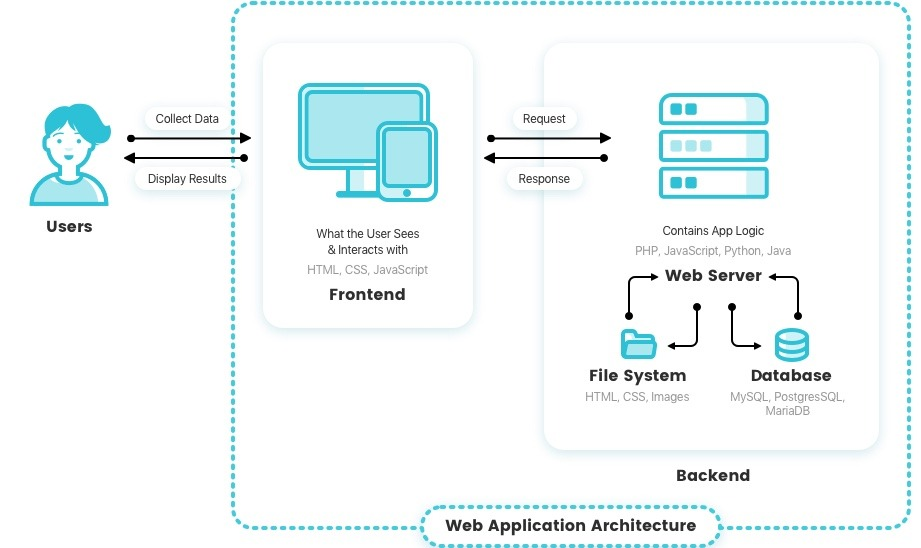
\includegraphics[scale=0.4]{images/architektura}
	\caption{Webes alkalmazás architekúrája}
	\label{abra:Architektura}
\end{figure}

\section {A React JavaScript keretrendszer}

Az elmúlt években a React JS jelentős népszerűségre tett szert a webfejlesztés területén. A React egy nyílt forráskódú JavaScript keretrendszer, amelyet a Facebook (Meta) fejlesztett ki, és célja a felhasználói felületek könnyű és hatékony megvalósítása. A React alapvetően egy komponens alapú megközelítést kínál, amely lehetővé teszi a fejlesztők számára, hogy újra felhasználható, önálló építőelemeket hozzanak létre, amelyeket könnyedén kombinálhatnak egymással a komplexebb felhasználói felületek elkészítése érdekében.

A React (\ref{abra:reactLogo}) rendkívül népszerűvé vált a fejlesztők körében számos előnye miatt. Elsőként említhetjük a hatékony Virtual DOM implementációját, amely lehetővé teszi az alkalmazások gyors és hatékony frissítését. A Virtual DOM a weboldal megjelenítéséhez használt valós DOM virtuális reprezentációja. Amikor változás történik az adatokban, a React a Virtual DOM-on keresztül kiszámítja az optimális frissítéseket, majd ezeket a változtatásokat csak a valós DOM-ra alkalmazza. Ez a megközelítés jelentős sebességjavulást eredményez a webalkalmazásokban.

\pagebreak
A második fontos előny a komponens alapú megközelítés, amely lehetővé teszi a fejlesztők számára a komponensek újra felhasználását és a kód modularizációját. A React komponensek önmagukban zárt egységek, amelyek különböző feladatokat elláthatnak a felhasználói felületeken, például gombok, űrlapok, listák stb. Az egyedi komponensek könnyedén kombinálhatók egymással, így a fejlesztőknek nem kell újra megírniuk a kódot, hanem egyszerűen felhasználhatják a meglévő komponenseket.

Emellett más technológiai óriások is felfedezték a React előnyeit. Például a Netflix, a PayPal, az Airbnb és a Dropbox is a React-et használja az alkalmazásaik fejlesztéséhez. Ezek a vállalatok magas forgalommal és komplex felhasználói felületekkel rendelkeznek, és a React segítségével könnyedén kezelhetik ezeket a kihívásokat.

Az open-source software (OSS) közösség is hozzájárult a React népszerűségének növekedéséhez. Számos harmadik fél által (Third party) készített könyvtár és eszköz érhető el a React-hez, amelyek további lehetőségeket kínálnak a fejlesztőknek. Ilyen példa a Redux, amely egy állapotkezelő könyvtár, vagy a React Router, amely segít az alkalmazások útvonalainak kezelésében.

A JavaScript önmagában egy típusfüggetlen programozási nyelv, de egyes keretrendszerek, mint a Next.js, a Microsoft által kifejlesztett TypeScript nyelvet használják, amely már megengedi a beépített és személyre szabott típusok használatát.

\begin{figure}[!h]
	\centering
	
\includegraphics[scale=0.02]{images/reactLogo}
	\caption{React logó}
	\label{abra:reactLogo}
\end{figure}

\section {A Google Firebase platform}

Mivel a React a webes alkalmazások frontend-jének fejlesztésére szolgál, szükségem volt egy backend szerverre és egy adatbázis-kezelő rendszerre, amely kiszolgálja a frontend-et, a Google által fejlesztett Firebase platformot és API-kat építettem be az alkalmazásba.
A Google Firebase (\ref{abra:firebaseLogo}) egy teljes körű fejlesztői platform, amely különféle eszközöket és szolgáltatásokat kínál a fejlesztőknek, hogy könnyedén hozzanak létre, teszteljenek és üzemeltessenek webes és mobilalkalmazásokat.

A Firebase Realtime Database egy NoSQL alapú adatbázis, amely valós idejű adatszinkronizációt tesz lehetővé az alkalmazások között. Ez azt jelenti, hogy az adatok automatikusan frissülnek minden csatlakozott eszközön, így a felhasználók valós idejű élményt élvezhetnek. Ez különösen hasznos például csevegőalkalmazások vagy valós idejű játékok fejlesztésekor. 

A Firebase Authentication lehetővé teszi a felhasználók egyszerű és biztonságos hitelesítését. Támogatja az e-mail és jelszó, a szociális média hitelesítés (pl. Google, Facebook, Twitter) és más autentikációs módokat is. A Firebase emellett lehetőséget biztosít a felhasználói fiókok-, profilok kezelésére és jogosultságkezelésre is. 

\pagebreak
A Firebase Cloud Storage segítségével könnyedén tárolhatóak és kezelhetőek az alkalmazásban használt fájlok, például képek, hangfájlok vagy videók. Az egyszerű API-k lehetővé teszik a fájlok feltöltését, letöltését és megosztását. Emellett a Firebase Hosting segítségével egyszerűen és gyorsan ki lehet szolgálni az alkalmazás statikus fájljait a világ bármely pontjáról.

A Storage Bucket-ek egy nagy tárolóhelyet jelentenek a fájlok (például képek, hangfájlok, videók stb.) biztonságos tárolására a felhőben. A Firebase Storage lehetővé teszi a fájlok feltöltését, letöltését, törlését és megosztását egyszerű API-k segítségével. Emellett automatikusan kezeli a fájlok hozzáférési jogosultságait és a CDN révén biztosítja a gyors és megbízható fájlletöltést a felhasználóknak.

\begin{figure}[!h]
	\centering
	
\includegraphics[scale=0.1]{images/firebaseLogo}
	\caption{Firebase logó}
	\label{abra:firebaseLogo}
\end{figure}

\section {Az AES titkosítás}
\subsection {Bevezető}

Az AES egy blokk titkosítási algoritmus, amelyet két belga kriptográfus tervezett 1997-ben. Az algoritmus az 1990-ben meghirdetett nyilvános pályázat nyertese lett, és 2001-ben a NIST (National Institute of Standards and Technology) elfogadta az Egyesült Államok kormányzati szervezetei számára ajánlott titkosítási szabványnak. Mivel az említett pályázat elbírálása publikusan történt, ezért valószínűleg nem történt befolyás a díj megítélését illetően. Az algoritmus egy változata a Rinjdael algoritmusnak, amely eredetileg több blokkmérettel is dolgozott és ebből választották ki az AES-t, amelynek blokkmérete 128 bit \cite{AES}.

A blokk mérete 128 bit, és a kulcs mérete lehet 128, 192 vagy 256 bit. Az AES hatékonysága körülbelül 109 Mb/s, amely természetesen függ az adott hardver tulajdonságaitól, és szakértők szerint a 256 bites kulcsméret biztonsága "örök" időkre szól.

Az algoritmus nem használja a Feistel-sémát, mint a DES (Data Encryption Standard), hanem iteratív szerkezetű. Az algoritmus a kulcsméret alapján különböző számú körökben végzi a titkosítást, amelyekhez korkulcsokat generál. A 128 bites kulcs esetén a körök száma 10, a 192 bites kulcs esetén a körök száma 12, míg a 256 bites kulcs esetén a körök száma 14.

Az AES helyettesítést és permutációt alkalmaz a blokkon belül, és véges testek felett végez aritmetikai és műveletet. Az algoritmus térnyerésére az szolgált, hogy a művelet végzés egész számokkal történik, ezért a szerzők egy olyan algoritmust fejlesztettek, ahol az összeadás, kivonás, szorzás, osztás után is halmazbeli elemet kapunk. Az AES véges testként használja a bináris együtthatós polinomokat a GF(2\textasciicircum n) felett, ahol n = 8 fokszámnál kisebb.

Minden műveletet 8 biten végez, és az összes 30 irreducibilis polinom közül a következőt használja: $x\textasciicircum 8 + x\textasciicircum 4 + x\textasciicircum 3 + x + 1$. Az AES minden bájtot a $GF(2\textasciicircum 8) = GF(2)[x]/(x\textasciicircum 8 + x\textasciicircum 4 + x\textasciicircum 3 + x + 1)$ testelemeként kezel.

Az AES-t általában három algoritmus alkotja: a kulcsgenerálás, a titkosítás és a visszafejtés. Az AES a bemeneti 128 bites állapotot (state) egy 4x4-es mátrix formájában kezeli, és az algoritmus minden iterációja során helyettesítő és permutációs műveleteket végez el a blokkon belül \cite{Marton}.

\subsection {Az algoritmus elmélete}

Az algoritmus a bemeneti adatokat 128 bites blokkokra bontja. A bemeneti adatokat több körön keresztül módosítja míg el nem jutunk a titkosított adatig. A módosításokat az algoritmus több lépésben hajtja végre. Ezeket a lépéseket altranszformációknak nevezzük.

Az altranszformációk három típusúak lehetnek: AddRoundKey, SubBytes és ShiftRows. Az AddRoundKey lépés során az aktuális kör kulcsát XOR művelettel adja hozzá adatblokkhoz. A SubBytes lépés a bemeneti blokk minden elemén végigmegy egy előre meghatározott nemlineáris függvénnyel. A ShiftRows lépés során az adatblokk minden sorát egy bizonyos számmal rotáljuk.

Összességében az AES titkosítási algoritmus magába foglalja a bemeneti adatok blokkokra bontását, majd a bemeneti blokkokon végrehajtja az altranszformációkat több körön keresztül, amíg meg nem kapja a titkosított adatot. Az algoritmus célja az adatok biztonságos és hatékony titkosítása a megfelelő védelem érdekében.

\subsection{Alkalmazások és érdekességek}

\begin{itemize}
	\item Az AES algoritmusnak 128, 192 és 256 bites változatai vannak, amelyek mindegyike különböző szintű biztonságot nyújt.
	\item Az algoritmus rendkívül hatékony, amely lehetővé teszi a titkosított adatok nagy sebességű feldolgozását.
	\item Nyilvánosan elérhető és ingyenesen használható, ami azt jelenti, hogy bárki használhatja és integrálhatja az alkalmazásába.
	\item Az algoritmus számos könyvtárcsomagban van megvalósítva. Léteznek egyaránt publikus és privát forráskódok, amelyek közül néhány optimalizálva van a hardveres és szoftveres rendszerekhez.
	\item Az alkalmazása különböző területeken népszerű, például az online banki- és pénzügyi tranzakciókban, a VPN (Virtual Private Network) rendszerekben, a Wi-Fi hálózatokban, az adattároló eszközökön.
	\item Az AES használata akkor biztosít teljes biztonságot, ha azt együtt használják egyéb kriptográfiai primitívekkel, mint az RSA. A kulcsfontosságú védelmi rendszerekben, mint például a HTTPS, SSH vagy TLS, használnak több rétegű védelmi mechanizmusokat az AES kiegészítéseként.
	\item A 256 bites titkosítási kulcsokat sokkal nehezebb brute-force módon támadni, mint egy 128 bites kulcsot. Azonban az utóbbi is olyan hosszú időbe telik kitalálni, még hatalmas számítási kapacitás mellett is, hogy az előrelátható jövőben nem lesz probléma, mert egy támadónak is hatalmas számítási kapacitásra lenne szüksége a szükséges brute-force (nyers-erő módszere) generáláshoz.
	\item Azonban a 256 bites kulcsokhoz is több feldolgozási teljesítmény szükséges és hosszabb ideig tarthat a generálásuk. Amikor az energiafogyasztás problémát jelent, különösen kis eszközök esetében, vagy a késleltetés valószínű, a 128 bites kulcsok jobb választásnak számítanak.
\end{itemize}

\section {RSA kulcscsere protokoll}

Az \textbf{RSA (Rivest-Shamir-Adleman)} egy kriptográfiai algoritmus, amely nyilvános kulcsokkal dolgozik. Ezt a matematikai alapokon fekvő eljárást számos területen használják, mint a titkosítás, elektronikus aláírások és kulcscsere. Az RSA kulcscsere rendszerben mindkét félnek van egy \textbf{publikus}- és egy \textbf{privát} kulcsa. A nyilvános kulcsot a feladó közzéteszi, míg a privát kulcs titkos marad, amely csak a címzett számára ismert. Az üzenetek titkosításához a feladó használja a címzett nyilvános kulcsát, majd a címzett a saját privát kulcsával tudja megfejteni az üzenetet. Ez biztosítja a biztonságos kommunikációt, mivel csak a címzett képes elolvasni az üzenetet (\ref{abra:rsa}).

\begin{figure}[!h]
	\centering
	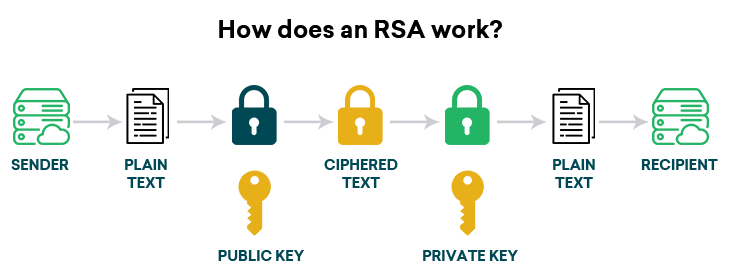
\includegraphics[scale=0.4]{images/rsa}
	\caption{RSA protokoll működése}
	\label{abra:rsa}
\end{figure}

A RSA protokoll alapvetően a prímtényezőkre bontás nehézségén alapul. A kulcsok mérete befolyásolja a rendszer biztonságát, azaz minél hosszabb a kulcs, annál nehezebb a faktorizáció, és így biztonságosabb a rendszer \cite{SZTE}.

Fontos megjegyezni, hogy a nagyobb kulcsok használata növeli a számítási időt és az erőforrásigényt, ezért a RSA rendszer lassabb lehet a titkos kulcsú kriptográfiához képest.

Az RSA-t a legtöbb esetben együtt használják olyan privát szimmetrikus kulcsú algoritmusokkal, mint az \textbf{AES} (Advanced Encryption Standard), \textbf{DES} (Data Encryption Standard), vagy a \textbf{Blowfish}. Az RSA titkosítja a szimmetrikus kulcsot, majd ezzel a titkosított kulccsal titkosítja az üzenetet. Ez azért hasznos, mert a szimmetrikus kulcsú algoritmusok hatékonyabbak a hosszú üzenetek titkosításában. Az F1 Ticket Managerben az RSA-t az AES-el együtt használóm a jegyek kódjainak titkosítására.

Az alkalamzásomban minden vásárlás esetén generálok egy egyedi RSA kulcspárt, amelyet a Google Firestore-ban tárolok a felhasználók rendeléseinek dokumentumában. Ez nagyban lassítja az alkalmazás sebességét, mivel minden rendeléskor történik kulcsgenerálás, ami önmagában is egy időigényes folyamat. Továbbá a hitelesítés folyamatában meg kell keresni a felhasználó rendelései között az adott egyedi azonosítóval ellátott rendelést és ezáltal a hozzá tartozó kulcsokat, valamint az \textbf{orders} dokumentumon belül az adott versenypályához tartozó rendeléseket, ahol hasonlóan az egyedi azonosító alapján tudja lekérni a rendszer a titkosított kódot.

Fontos megjegyezni, hogy a \textit{gyorsaság} és a \textit{biztonság} nagy mértékben befolyásolják egymást. Ennek értelmében ha egy rendszer biztonságos, akkor a veszíteni fog a teljesítményéből a bonyolult és adott esetekben sok matematikai számítás során. Ha viszont gyors, akkor az a rendszer kevésbé biztonságos.

Az \textit{F1 Ticket Manager}ben előtérbe helyeztem a biztonság mértékét a gyorsasággal szemben, mivel érzékeny adatokról van szó. Az alkalmazás teljesítményét ettől függetlenül lehet fejleszteni annak skálázásával, vagyis a szerverek mennyiségének és teherbírásuknak növelésével.

\section {Kutatási kérdések} \label{research}

Az alkalmazás fejlesztése során a következő kérdésekre próbáltam válaszokat keresni:
\begin{itemize}
	\item Hogyan lehet biztonságosabbá tenni az elektronikus jegyvásárlást és azok felhasználását?
	\item Mely technológiák segítségével lehet gyors és hatékony online üzletet tervezni és megvalósítani?
	\item Hogyan lehet a megvalósított rendszert hosszú távon karban tartani és felügyelni?
	\item Hogyan lehetséges a rendszer automatizálása valós időben?
\end{itemize}

\section {Célkitűzések} \label{scopes}

A kutatási kérdésekre keresett válaszok során felmerültek további kérdések, amelyek hozzájárulnak a céljaim pontosabb megfogalmazásában:
\begin{itemize}
	\item Hol és hogyan fogom tárolni a felhasználói- és alkalmazás adatokat?
	\item Hogyan fogom kezelni a felhasználói jogosultságokat, hogy minden felhaszáló csak a saját adataihoz férjen hozzá?
	\item Hogyan fogom megvalósítani a többlépcsős azonosítást a jegyek felhasználásásnál?
	\item Hogyan fogom eljuttatni a felhasználóknak a megvásárolt termék(ek)ről és azok azonosításához szükséges információkat? 
	\item Hogyan tudom a felületet felhasználóbaráttá tenni?
\end{itemize}

A megfogalmazott kérdések azt a legfontosabb célt hivatottak szolgálni, hogy egy kényelmes és megbízható alkalmazás jöjjön létre a felhasználók számára. Ennek megvalósításához szükséges szempont, hogy megbizonyosodjanak a felhasználók, hogy a felület használata nem félreérthető és nincsenek olyan működési aspektusok, amelyek zavarhatják a felhasználói élményt.

Az előbbiek elérésére a kisebb célok egy még pontosabb képet tudnak biztosítani számomra, hogy megfelelő ütemben haladjon a fejlesztés anélkül. hogy kimaradjanak fontos részletek.

A fent felsorolt kérdések felhívják a figyelmet arra a fontos tényezőre, hogy az egyre elterjedtebb körű internet használatának korszakában elengedhetetlen a felhasználók személyes adatainak a védelme. Ennek megvalósítására is érdemes számos megoldást kutatni és majd kiválasztani az alkalmazás szempontjából megfelelőt.

Továbbá a előzőek mellett megoldást kell kapjak arra a problémára, hogy a jelenleg is működő oldalak nagy része nem foglalkozik azzal a tényezővel, hogy egy elektronikus jegy nagyon sok veszélynek van kitéve és ennek ellenére nem alkalmaznak többlépcsős azonosítást a jegyek hitelesítésekor. Ennek egyszerűen az az oka, hogy bizonyos százalékban lassítaná a hitelesítési folyamatot és az eladók nem vállalnak felelősséget a jegyek esetleges elveszítése vagy ellopása esetén.

Végül de nem utolsó sorban fontos, hogy lehetőséget biztosítsak az alkalmazás viselkedésének monitorizálására, valamint az alkalmazás továbbfejleszthetőségére. Az alkalmazás működésének megfigyelése során olyan hibákról és ötletekre kaphatok visszajelzést, amivel tudom biztosítani az alkalmazás hosszútávú karbantartását és továbbfejlesztését.